\documentclass{article}

\usepackage[utf8]{inputenc}
\usepackage{graphicx}
\usepackage{tikz}
\usepackage{float}
\usepackage{wrapfig,lipsum}
\usepackage{svg}
\usepackage{mathtools}
\usepackage{tabu}
\usepackage{subcaption}
\usepackage[a4paper, total={6in, 8in}]{geometry}


\begin{document}


\newcommand{\vecthreeBF}[1]{\vec{\textbf{#1}}}
\newcommand{\vecthree}[1]{\vec{#1}}

\newcommand{\parDeriv}[2]{\frac{\partial #1}{\partial #2}}
\newcommand{\parDerivS}[2]{\frac{\partial^2 #1}{\partial #2^2}}
\newcommand{\derivS}[2]{\frac{d^2 #1}{d#2^2}}

\newcommand{\dotProdBF}[2]{\vecthreeBF{#1} \cdot \vecthreeBF{#2}}
\newcommand{\dotProd}[2]{\vecthree{#1} \cdot \vecthree{#2}}

\newcommand{\crossProdBF}[2]{\vecthreeBF{#1} \times \vecthreeBF{#2}}
\newcommand{\crossProd}[2]{\vecthree{#1} \times \vecthree{#2}}


\newcommand{\fromeq}[1]{\textit{equation \ref{eq:#1}}}
\newcommand{\fromeqs}[2]{\textit{equations \ref{eq:#1} and \ref{eq:#2}}}
\newcommand{\fromeqsth}[3]{\textit{equations \ref{eq:#1}, \ref{eq:#2} and \ref{eq:#3}}}

\newcommand{\fromfig}[1]{\textit{figure \ref{fig:#1}}}
\newcommand{\fromfigs}[2]{\textit{figures \ref{fig:#1} and \ref{fig:#2}}}
\newcommand{\fromsec}[1]{\textit{section \ref{sec:#1}}}

%----../../..++++.

%%%%%%

\section{Magnet Design} \label{sec:magnet_design}
Magnet design in rhodotron type accelerators depend heavily on the design of the cavities.
Because the limiting factors usually are frequency and total volume of the accelerator, magnet design parameters are considered after cavity design has been completed.
Considering the nature of coaxial cavity, simplest path for beams inside magnets is major segment of a circle, which was used as the reference for following discussions.

\begin{figure}[H]
    \captionsetup[subfigure]{justification=centering}
    \captionsetup{justification=centering}
    \centering
    \begin{subfigure}{.5\textwidth}
      \centering
      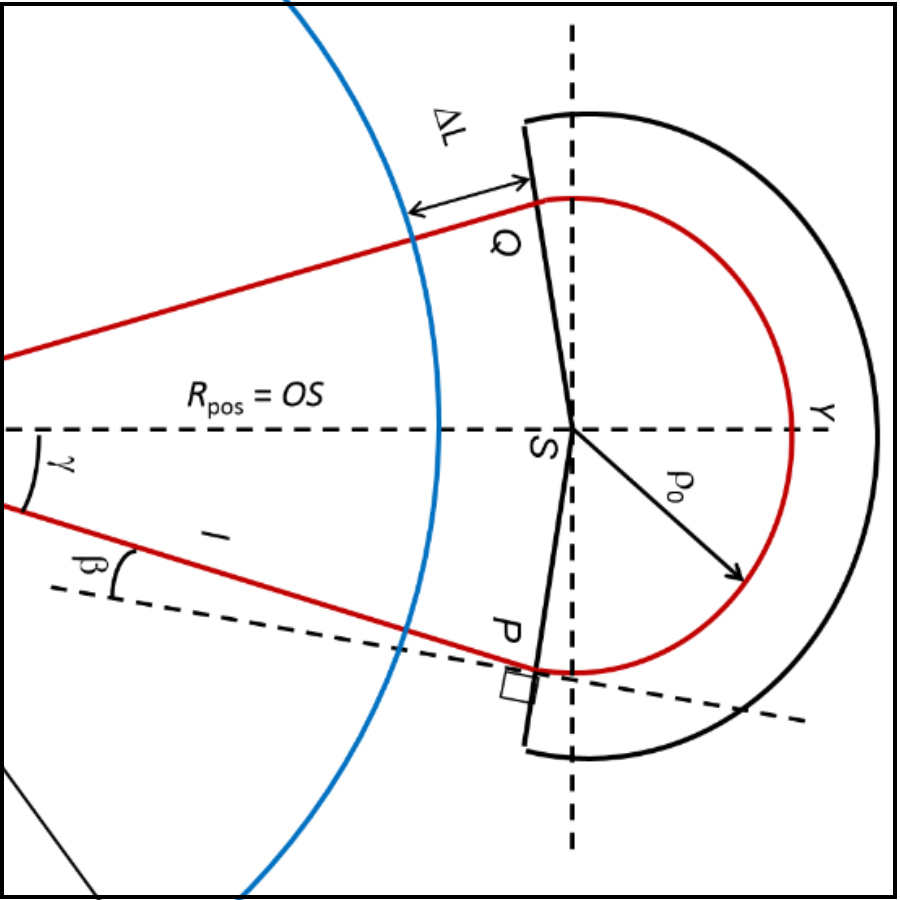
\includegraphics[width=.9\linewidth]{../../../figures/design/Ltot.png}
      \caption{Geometry of the outside trajectory \\ of a rhodotron \cite{cite:rhodo_design}}
    \end{subfigure}%
    \centering
    \begin{subfigure}{.5\textwidth}
      \centering
      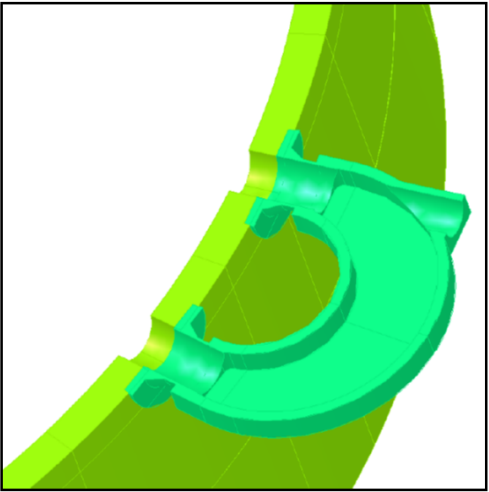
\includegraphics[width=.9\linewidth]{../../../figures/design/tt300_mag.png}
      \caption{Modeling of the outside trajectory \\ of a rhodotron (TT300) \cite{cite:rhodo_design}}
    \end{subfigure}
    \caption{From "Design and Simulation Tools for the \\ High-Intensity Industrial Rhodotron Electron Accelerator," \\by W.Kleeven, M.Abs, J.Brison, E.Forton, J.Hubert and J.Van de Walle}
    \label{fig:magnet_design_illustrations}
\end{figure}

In rhodotron accelerators, magnets are used for not only guiding the electron beam to desired path, but also for syncronizing them with the RF field in the cavity. 
This syncronization, also called phase stability, is the fundamental constraint of magnet design. 
Time spent outside of the cavity should be precisely tuned to maximize acceleration in the succeeding pass. 

Two different approaches have been used to achieve phase stability.
These approaches are discussed further in the following sections.

\subsection{$n\lambda$ Technique} \label{sec:n_L_technique}

First approach for phase stability considiration assumes that from the start of the current pass, $\beta_{avg} \approx 1$ for a synchronous particle. 

To maintain the phase synchronization, a particle that started the current pass at $t=0$, should start the next pass at $t=nT$, where $n$ is an integer and $T$ is the period of RF field inside cavity.
As discussed earlier, by assuming the electron is traveling at $c$, phase stability can be achieved by designing the whole trajectory to be $n \lambda$, where $\lambda$ is the wavelength of the RF field. 
In other words, total trajectory of synchronous particle needs to satisfy the following equality;
\begin{equation*}
    L_{pass} = n \lambda
\end{equation*} 
Since $n>1$ would require unnecessarily long and expensive beam guide and magnets, $n=1$ is the most efficient choice.
\begin{equation}
    L_{pass} = \lambda
\end{equation} 

\begin{figure}[H]    
    \centering
    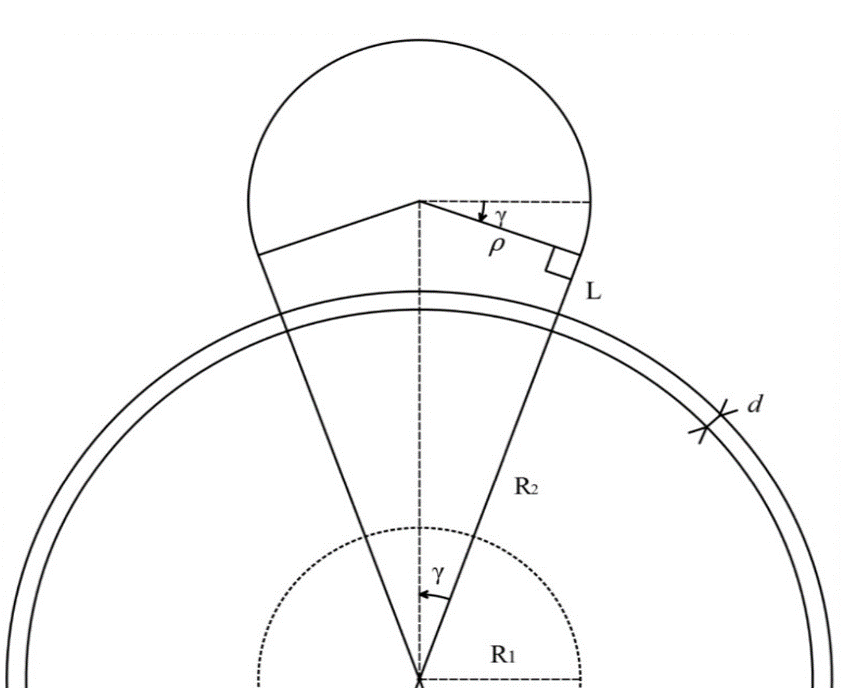
\includegraphics[width=.8\linewidth]{../../../figures/design/magnet_design.png}
    \caption{Trejectory of a particle in single pass}
    \label{fig:magnet_design}
\end{figure}

From \fromfig{magnet_design}, where $\gamma$ is half the angle between trajectories of successive passes, $\rho$ is the radius of the circular path inside magnet, $L$ is the length of the magnet guide, $d$ is the thickness of the cavity wall;
\begin{eqnarray}
    L_{in} &=& 2R_2 \nonumber\\
    L_{out} &=& 2L + 2d + (\pi + 2\gamma)\rho \nonumber \\
    L_{pass} &=& L_{in} + L_{out}  \nonumber \\
    \lambda &=& 2R_2 + 2d + 2L + (\pi + 2\gamma)\rho \label{eq:magnet_lambda_constraint}
\end{eqnarray}

After the cavity design is complete, only $L$, $\gamma$ and $\rho$ remain, which are the design parameters of magnets.
Observing the \fromfig{magnet_design} and using \fromeq{magnet_lambda_constraint},

\begin{eqnarray}
    tan(\gamma) &=& \frac{\rho}{R_2 + d + L} \nonumber \\
    \rho &=&  tan(\gamma) (R_2 + d + L) \nonumber\\
    2\rho &=& tan(\gamma) (\lambda - (\pi + 2\gamma)\rho) \nonumber\\
    \rho (2 + tan(\gamma)(\pi + 2\gamma)) &=&  tan(\gamma) \lambda \nonumber\\
    \rho &=& \frac{\lambda}{\pi + 2\gamma + \frac{2}{tan(\gamma)}} \label{eq:magnet_rho_constraint} \\
    L + d &=& \frac{\rho}{tan(\gamma)} - R_2 \label{eq:magnet_L_constraint}
\end{eqnarray}

\textit{Equations \ref{eq:magnet_rho_constraint} and \ref{eq:magnet_L_constraint}} define 2 constraints. As already discussed, it has been assumed that cavity design is set (\textit{i.e} $R_2$, $\lambda$, $d$ are already defined).
Therefore only the magnet design parameters $\rho$, $\gamma$ and $L$ are left. Together with the constraints, one free variable defines the whole magnet design. 
Considering the importance of $\gamma$ for maximum number of possible passes, it will be used as the free magnet design variable in the further discussions.


\subsection{$L_{out}$ Parameter Sweep} \label{sec:parameter_sweep}

As mentioned previously in \fromsec{n_L_technique}, \fromeq{magnet_lambda_constraint} assumes that the particles are fast enough so that $\Delta t_{pass} \approx n T$. 
This assumption is not guaranteed however, especially in the first few passes if the particles are not accelerated enough. 
This scenario can happen when RF power is not sufficiently high. 

Consider an RF supply with $f=1$ GHz, $P=50$ kW. Using \fromeq{W_total_gain_pottier}, 
after the first pass the synchronous electron that entered the accelerator with $40$ keV and $\phi=15^\circ$ phase lag,
\begin{eqnarray*}
    W_{gain} &=& 2.14\times0.2998^{1/4}\times 50000^{1/2} = 354keV \\
    W_{total} &=& 394 keV \\
    \beta_{40keV} &\approx& 0.374 \\
    \beta_{394keV} &\approx& 0.825
\end{eqnarray*}
It is clear that $\beta_{avg}$ is not fast enough to sustain phase stability if the magnet is designed for $\beta = 1$. 
For these cases, \fromeq{magnet_lambda_constraint} fails to deliver phase stability.
Another approach for designing a magnet would be to find a new constraint, $K$ for total path length.
\begin{eqnarray*}
    L_{pass} &=& K \\
    L_{in} + L_{out} &=& K
\end{eqnarray*}

Since $L_{in}$ is set previously from cavity design, we can remove it from our equation and continue with
\begin{equation} \label{eq:mag_sweep_constraint}
    L_{out} = K
\end{equation}

To start, an optimization criteria for the following pass such as
\begin{itemize}
    \item Ensure the phase stability of the synchronous electron
    \item Maximize the energy gain of the synchronous electron
    \item Minimize the energy spread of the beam
    \item Minimize the phase lag spread of the beam
    \item All of the above with decided weights
\end{itemize}
needs be selected. Using a simulation software such as \textit{CST Studio Particle Module}, the optimum value of $K$ for the criteria can be found by simulating for different values of $K$ (\textit{sweeping}) and analyzing the results.
This process can be repeated for each magnet until the desired beam characteristics in the end of the accelerator are achieved.

However, one caviat of this technique is that, available simulation softwares are not well suited for this kind of process. As mentioned above, \textit{CST Studio Particle Module} has a \textit{parameter sweep} functionality.
But the calculation times are too slow to be useful in this particular problem. \textit{A custom built software offering magnet optimizing sweep functionality will be discussed in the following chapter.}


%%%%%%


\end{document}